\newpage\section{Demonstration of the Artifact}

In order to validate the conceptualized artifact and to show its functionality, an experimental setup from a real study in the field of data analytics is exemplarily implemented with the conceptualized artifact. For this purpose, the study of S. Krakowski et al. (2022) is implemented using the conceptualized artifact. The 2022 study researches changes in the origin of competitive Advantages through the rise of Artificial intelligence. For this, they use a case study on chess tournaments to explore what impact \ac{ai} has on competitive advantage (\cite{Krakowski.2022}). Although the methodological experimental design of this article is perfectly fine, the test could have been done by experiment. According to B. Gniewosz (2011) an experiment would even have been the preferred methodology in this field (\cite{Gniewosz.2011}) and the authors themselves note that further research in this area should be conducted through experiments (\cite{Krakowski.2022}). Therefore, this study is a perfect candidate to validate the conceptualized artifact.
Nonetheless, it must additionally be noted that the artifact's implementation of the study is merely a sample implementation.
Figure \ref{fig:uiScreens} shows the four \ac{ui} Activities of the final artifact implementing the study of S. Krakowski et al. (2022). For this purpose, a custom activity (Subfigure \ref{subfig:ChessGame}) was created that contains a chess game that can be played between two people. Figure \ref{subfig:chooseTestSubject2}, \ref{subfig:Questionair2} and \ref{subfig:InfoScreen2} show the conceptualized standard functionalities of the artefact. The individual fields that are visible in the \ac{ui} are dynamically filled with data from the corresponding data sources. The experiment data specifies the order of the screens as follows (1) Information Screen (2) Participant Selection Screen (3) Questionnair Screen (4) Custom Chess Game Activity. The participant data contains dummy data of five participants that have no prior information filled out about them. The application is emulated on a Pixel 4 XL API 30.

\begin{figure}[htbp]
    \centering
    \begin{subfigure}[b]{0.25\textwidth}
        \centering
        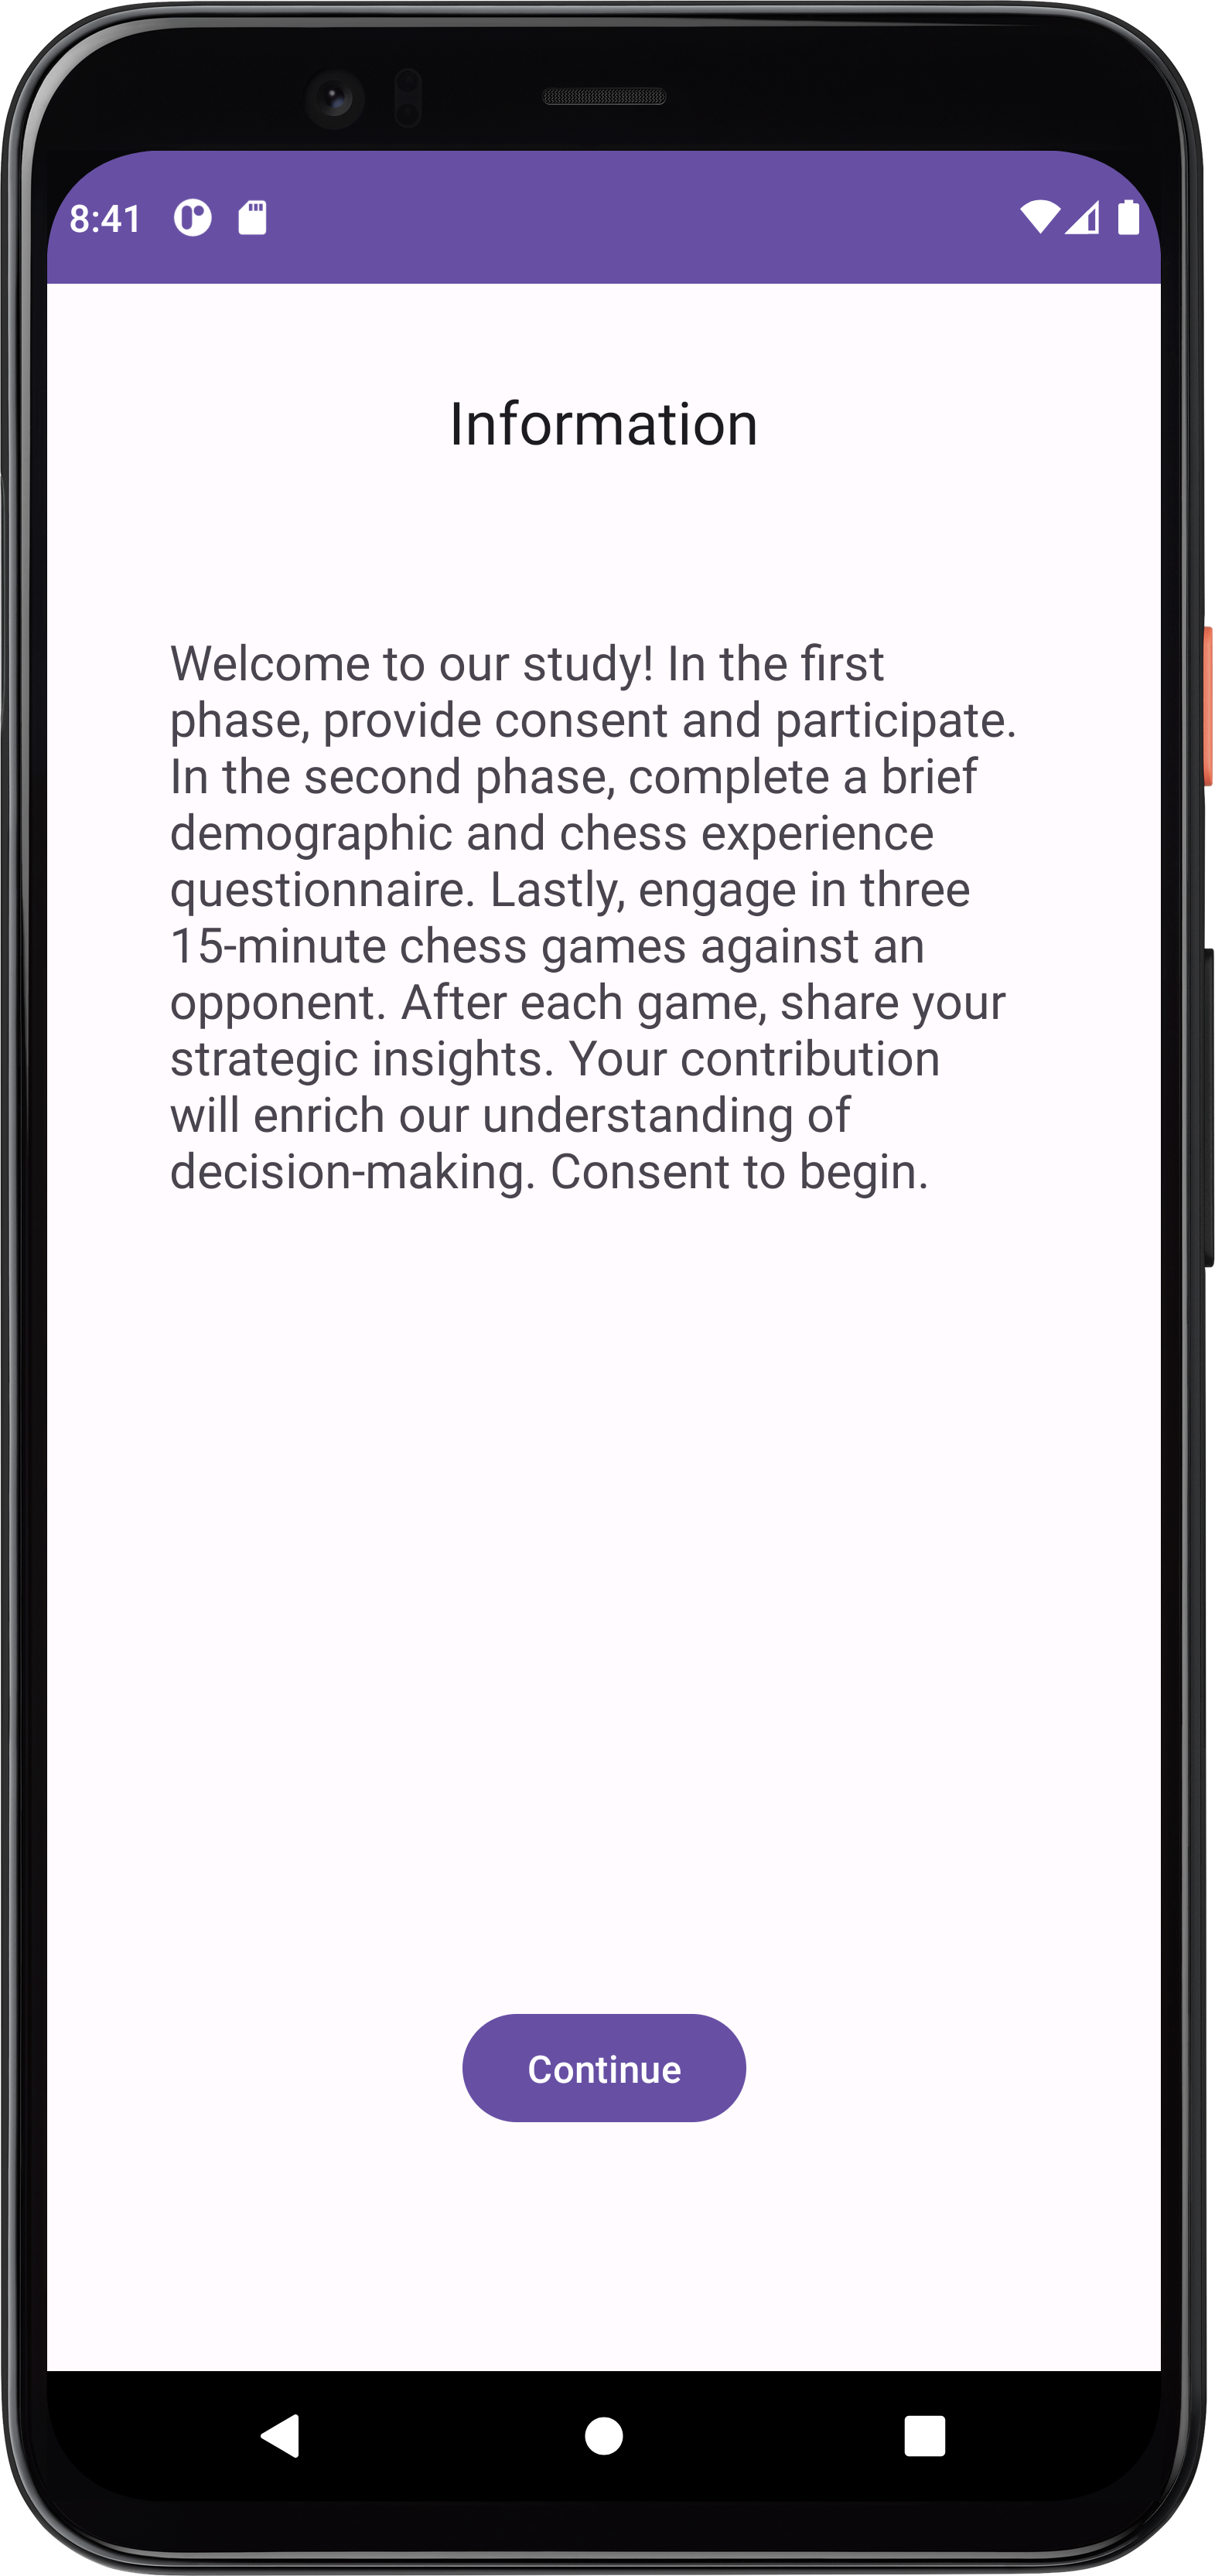
\includegraphics[width=\textwidth]{content/06_demonstration_of_the_artifact/Screenshot_InfoScreen.png}
        \caption{Choose subject step}
        \label{subfig:chooseTestSubject2}
    \end{subfigure}
    %\hfill
    \hspace{1cm}
    \begin{subfigure}[b]{0.25\textwidth}
        \centering
        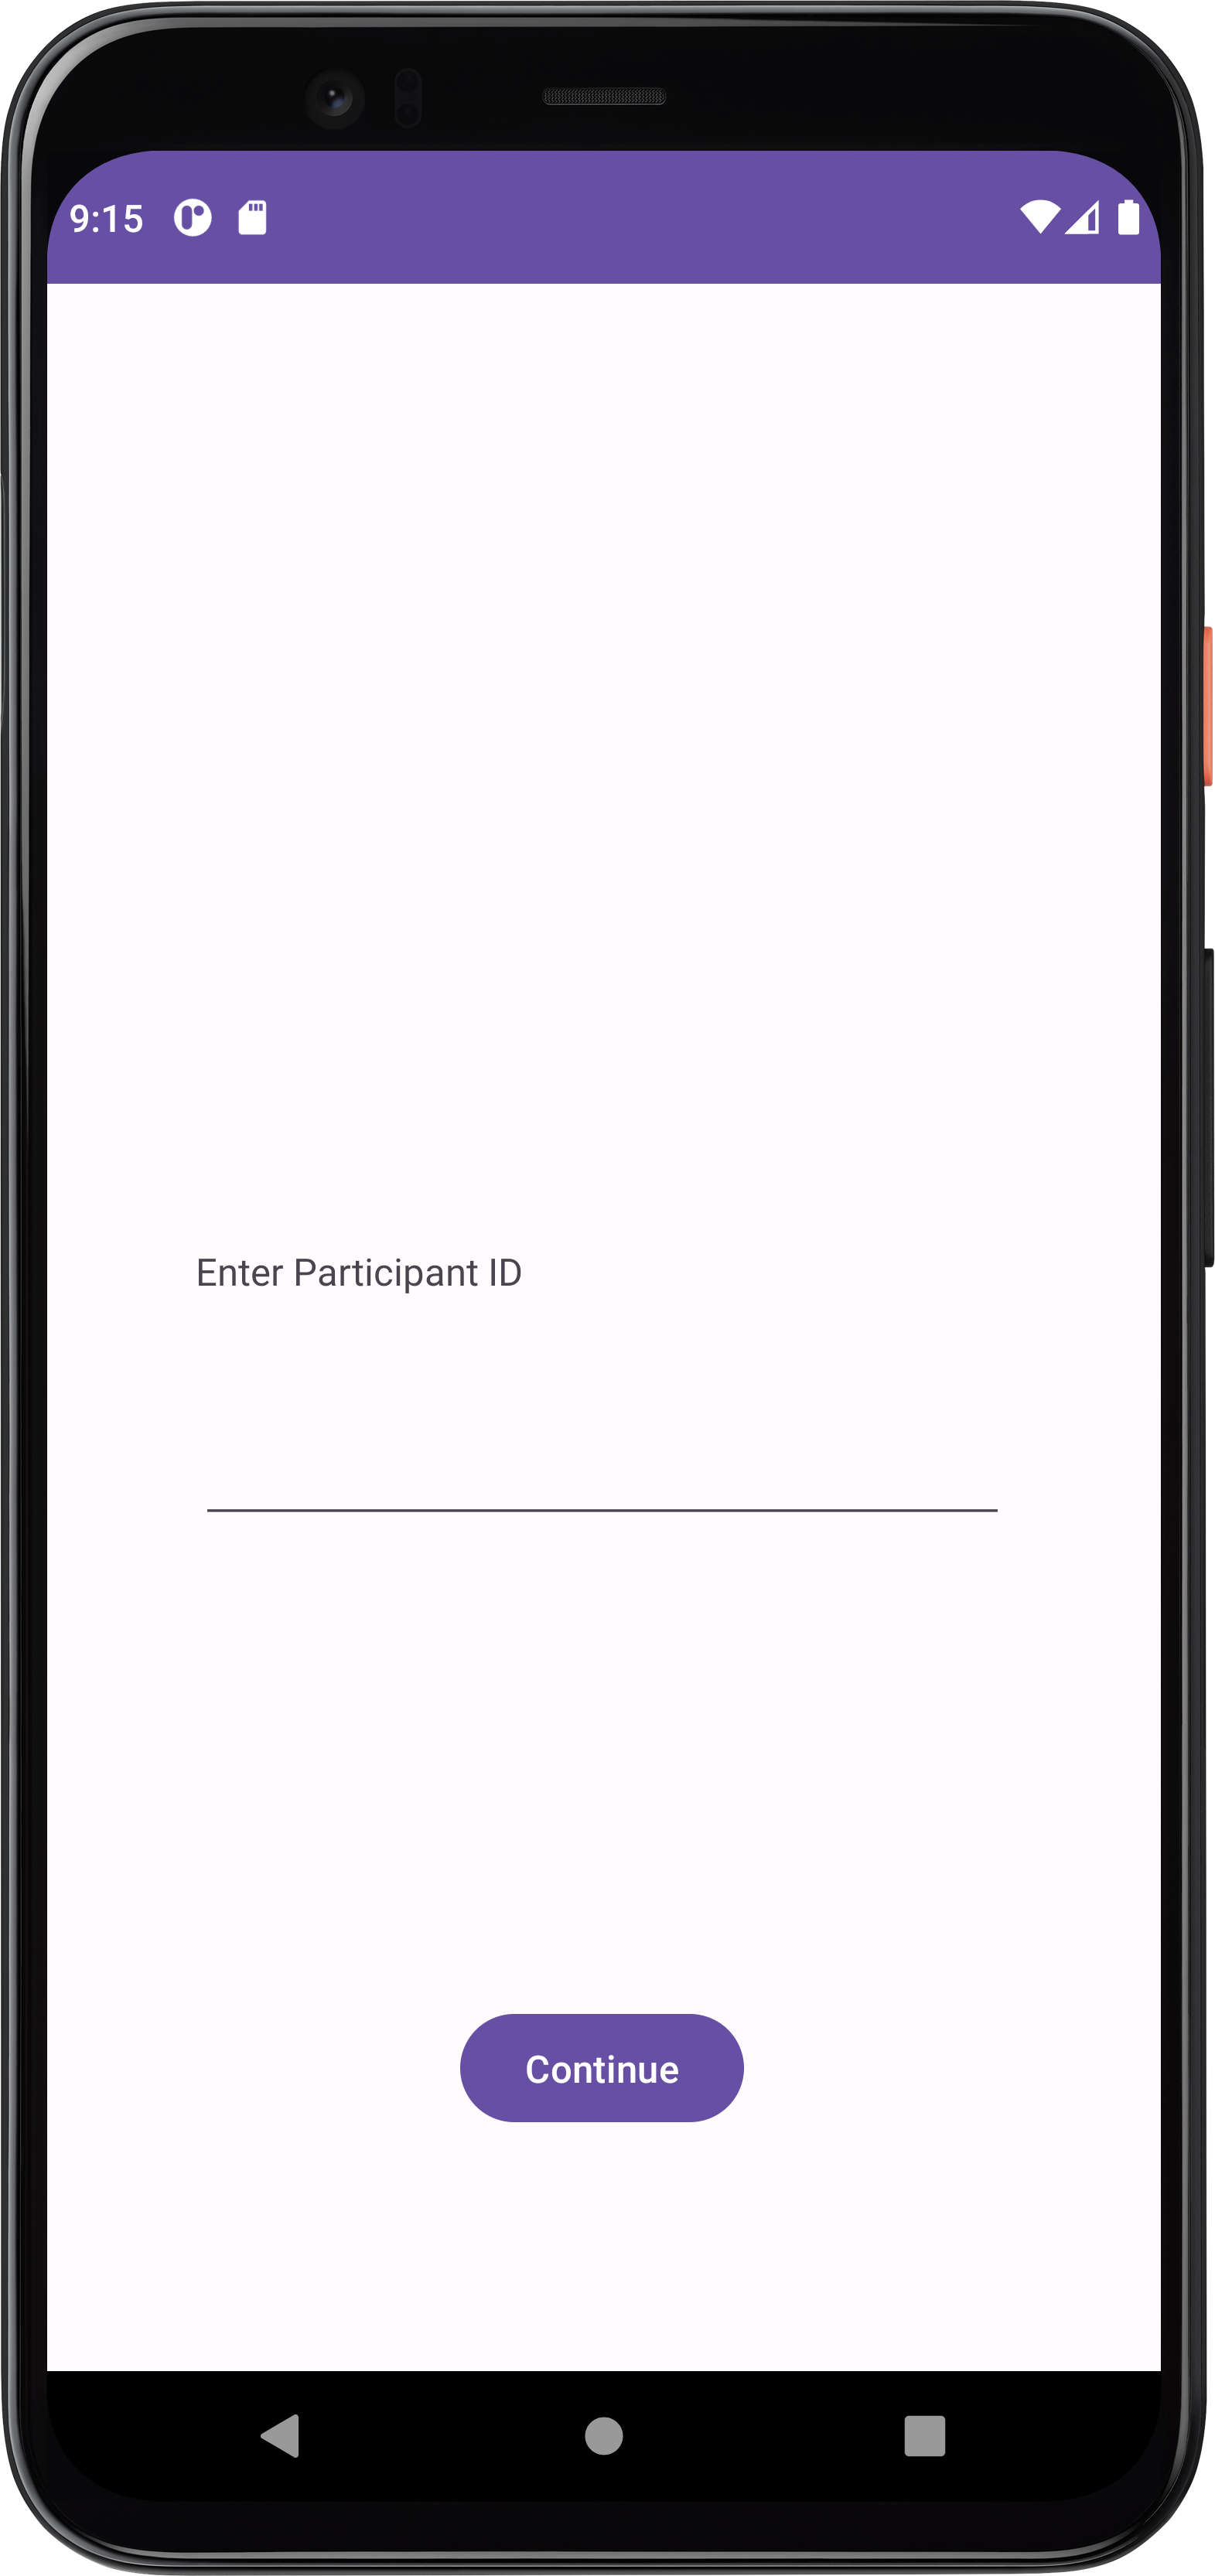
\includegraphics[width=\textwidth]{content/06_demonstration_of_the_artifact/Screenshot_ParticipantSelectionScreen.png}
        \caption{Questionair step}
        \label{subfig:Questionair2}
    \end{subfigure}
        %\hfill

%\end{figure}
\vspace{1cm}
%\begin{figure}[htbp]
  %  \centering
    \begin{subfigure}[b]{0.25\textwidth}
        \centering
        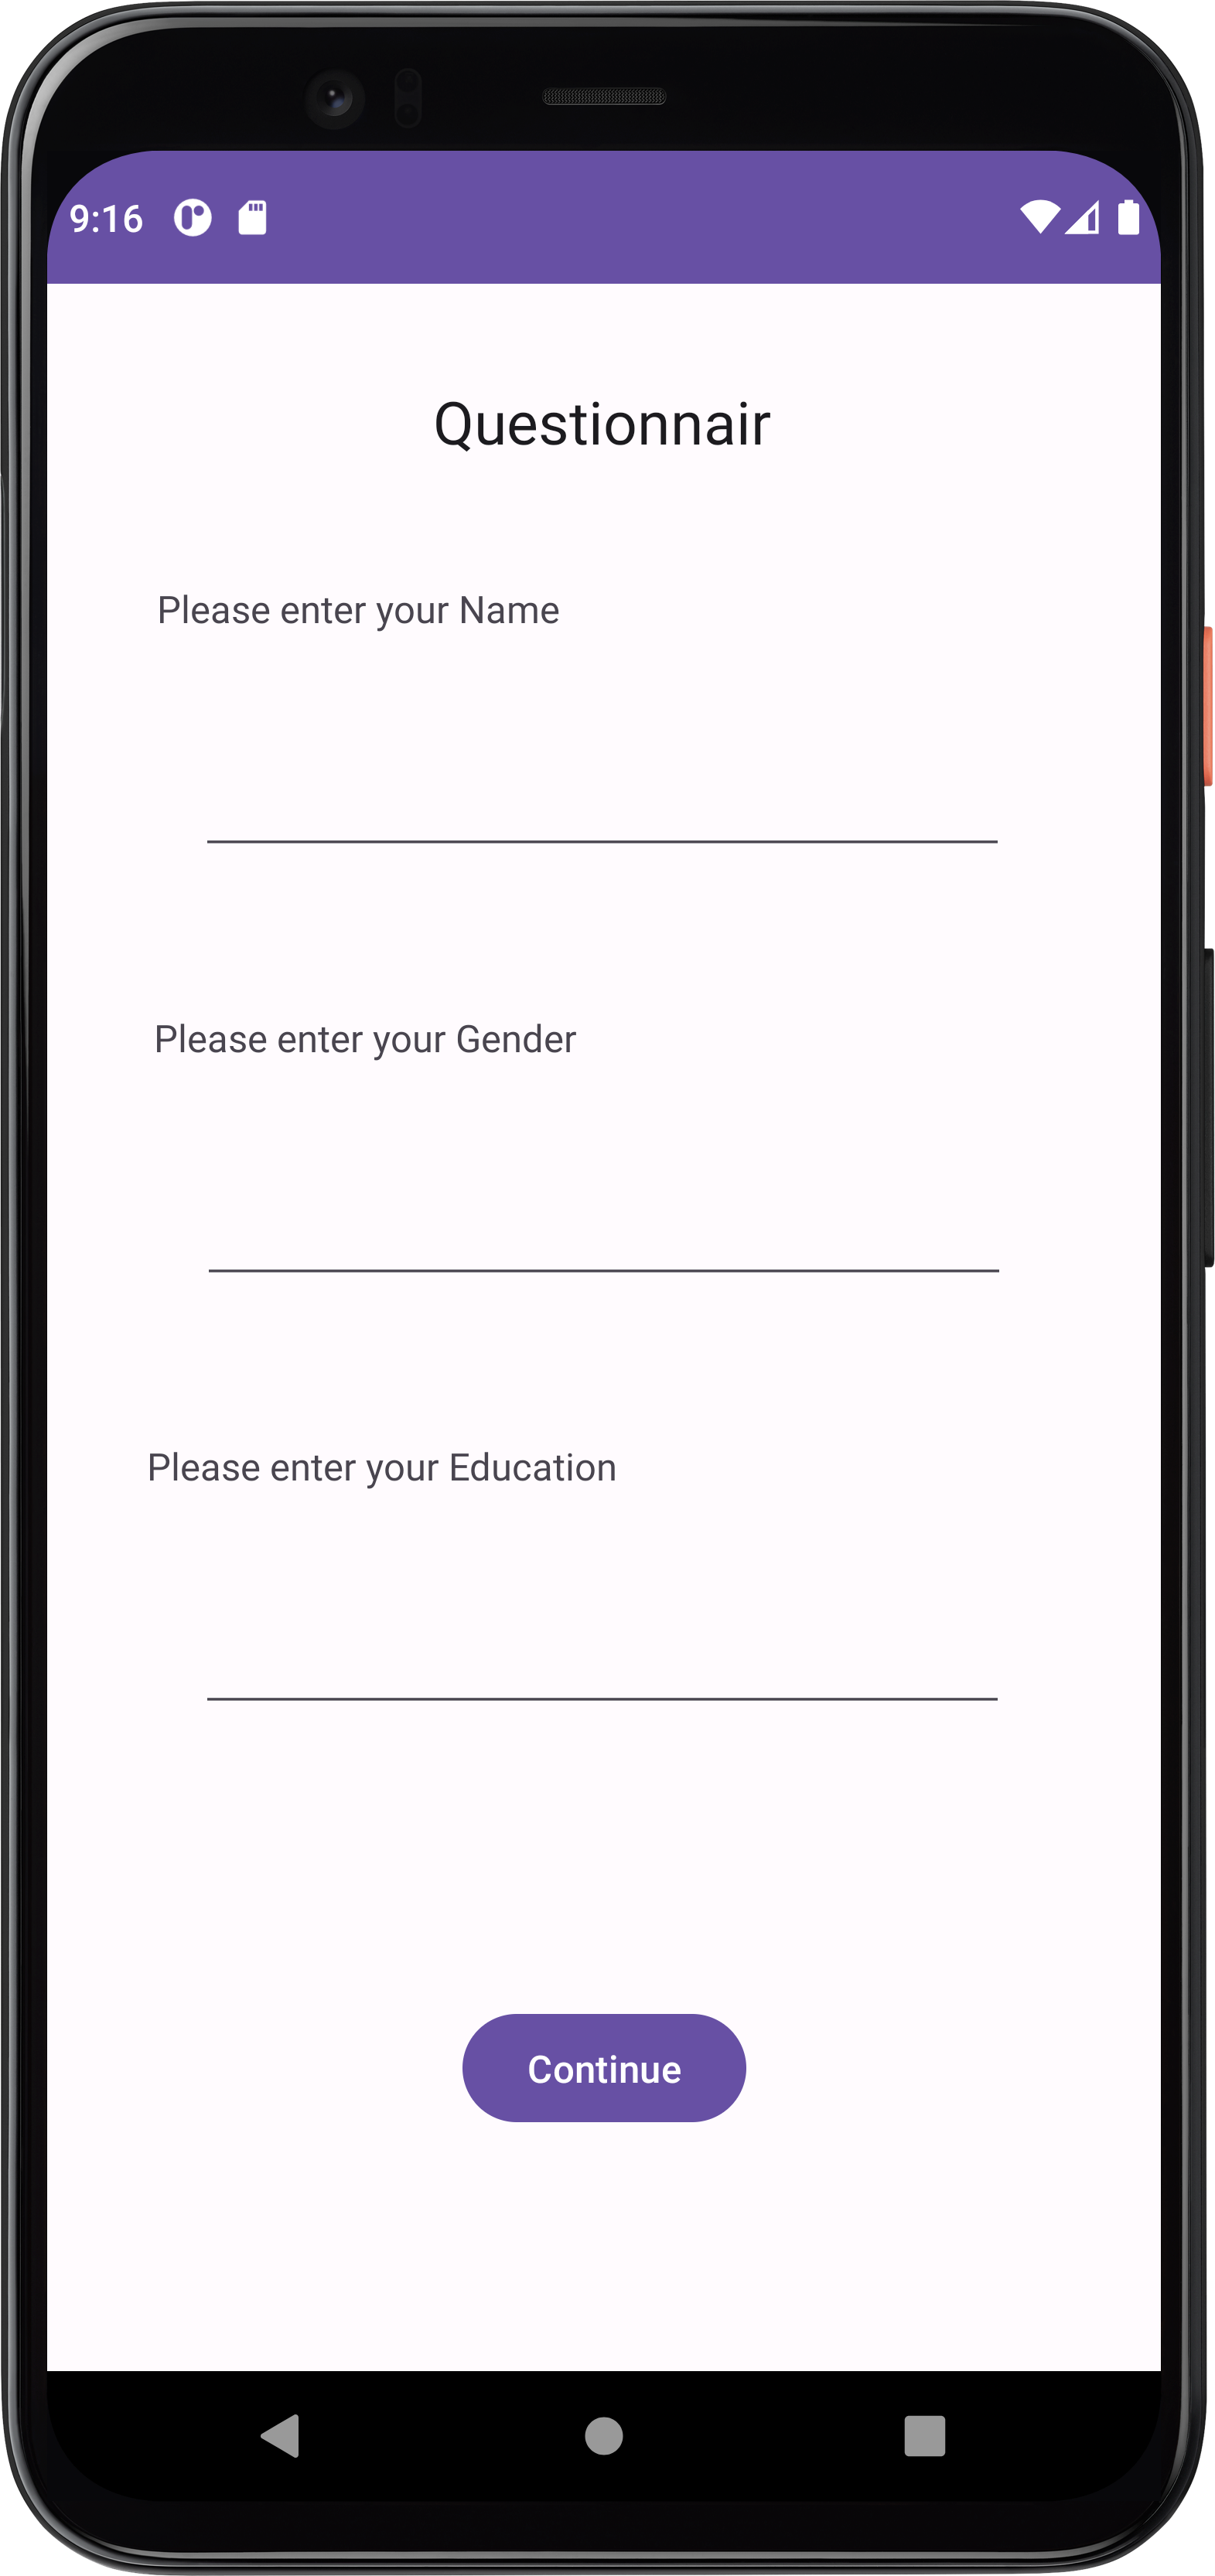
\includegraphics[width=\textwidth]{content/06_demonstration_of_the_artifact/Screenshot_QuestionnairScreen.png}
        \caption{Info screen step}
        \label{subfig:InfoScreen2}
    \end{subfigure}
    %\hfill
    \hspace{1cm}
    \begin{subfigure}[b]{0.25\textwidth}
        \centering
        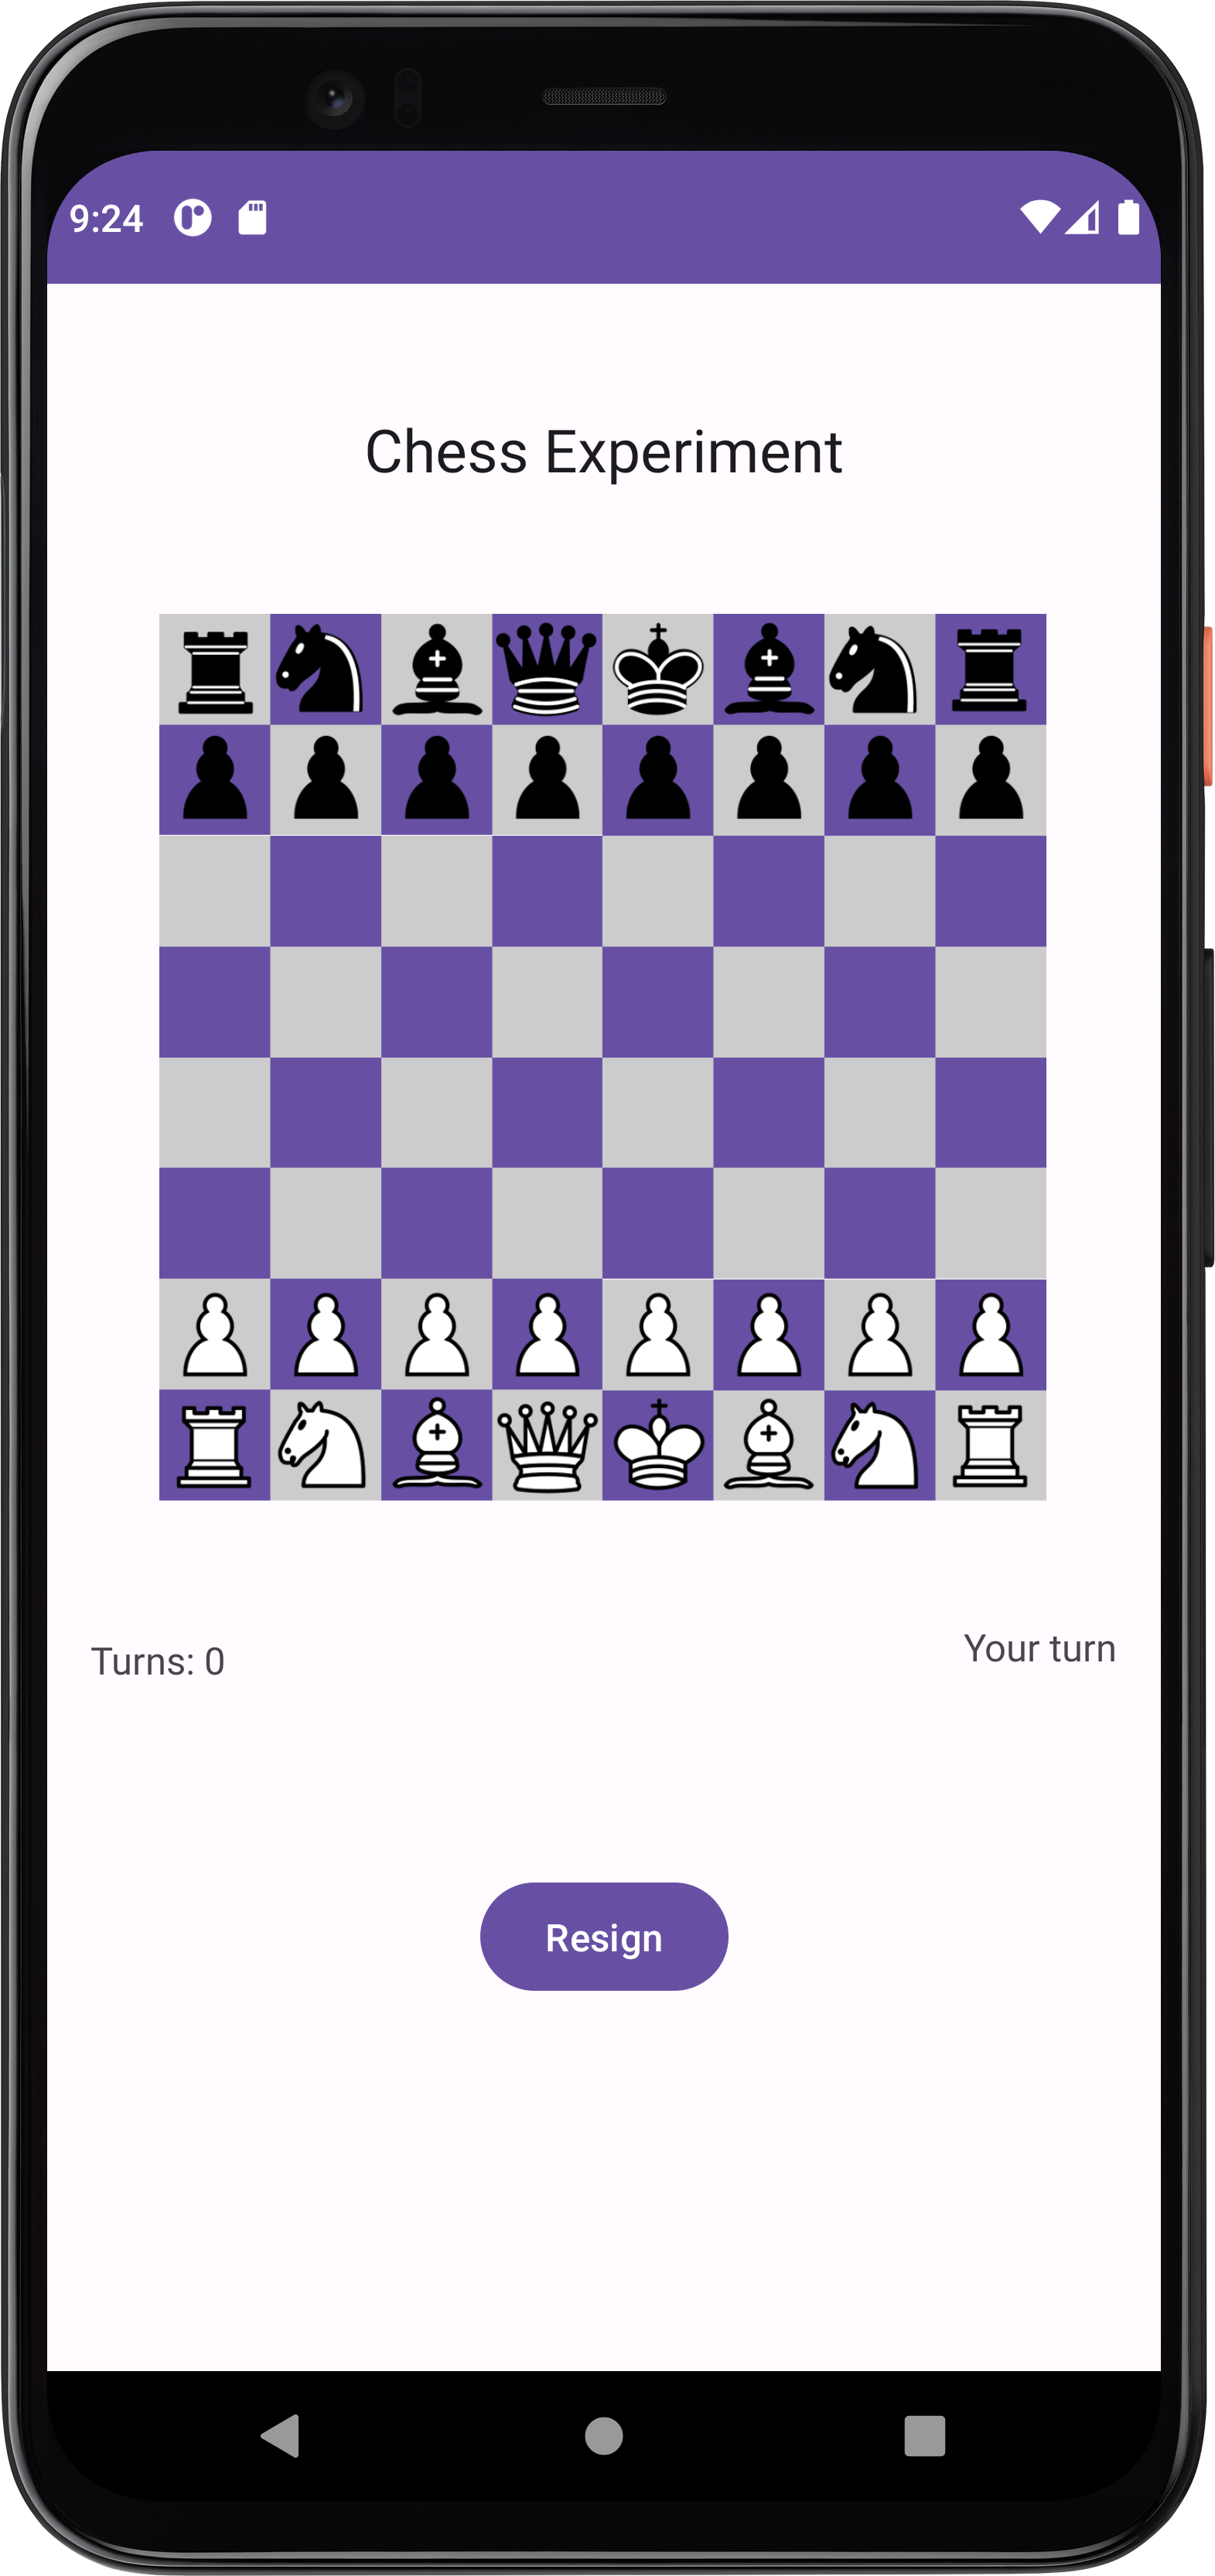
\includegraphics[width=\textwidth]{content/06_demonstration_of_the_artifact/Screenshot_Chess.png}
        \caption{Chess game}
        \label{subfig:ChessGame}
    \end{subfigure}
    \caption{User Interface Implementation}
    \label{fig:uiScreens}
\end{figure}

For changing or adding the individual \enquote{experiment steps} of the application or to change the questions within the questionnair step, only the experiment or participant data must be changed, without the need for additional coding, showcasing the simplicity and reusability of the artefact. The same applies to the Information Screen. New experiments can build on the existing UseCases in the domain layer and extend them in the course of object-oriented programming. If additional experiment steps contain \ac{ui} interactions, these are implemented via new Android Activities. The name of the activity must then only be stored in the experiment data as a string in order to call it. The full program code can be found in the Github repository at: \textit{https:\/\/github.com\/schneemax\/master\_thesis}